%%%%%%%%%%%%%%%%%%%%%%%%%%%%%%%% 
% Compile with
% pdflatex --shell-escape -synctex=1 -interaction=nonstopmode FILENAME.tex
% to convert it to png use:
% convert -density 300 -transparent white FILENAME.pdf FILENAME.png
%%%%%%%%%%%%%%%%%%%%%%%%%%%%%%%% 

\documentclass{standalone}

\usepackage[utf8]{inputenc}
\usepackage{tkz-fct}
\renewcommand{\familydefault}{\sfdefault}
\usepackage[scaled=1]{helvet}
\usepackage[helvet]{sfmath}
\everymath={\sf}
\usepackage{pagecolor}
\usetikzlibrary{calc,arrows,intersections,angles,quotes,patterns, backgrounds, shapes.misc}

\definecolor{AFLight}{HTML}{5CE0E6}
\definecolor{AFMiddle}{HTML}{51ADE5}
\definecolor{AFDark}{HTML}{0E4160}
\definecolor{AFOppo}{HTML}{FFB150}


\begin{document}

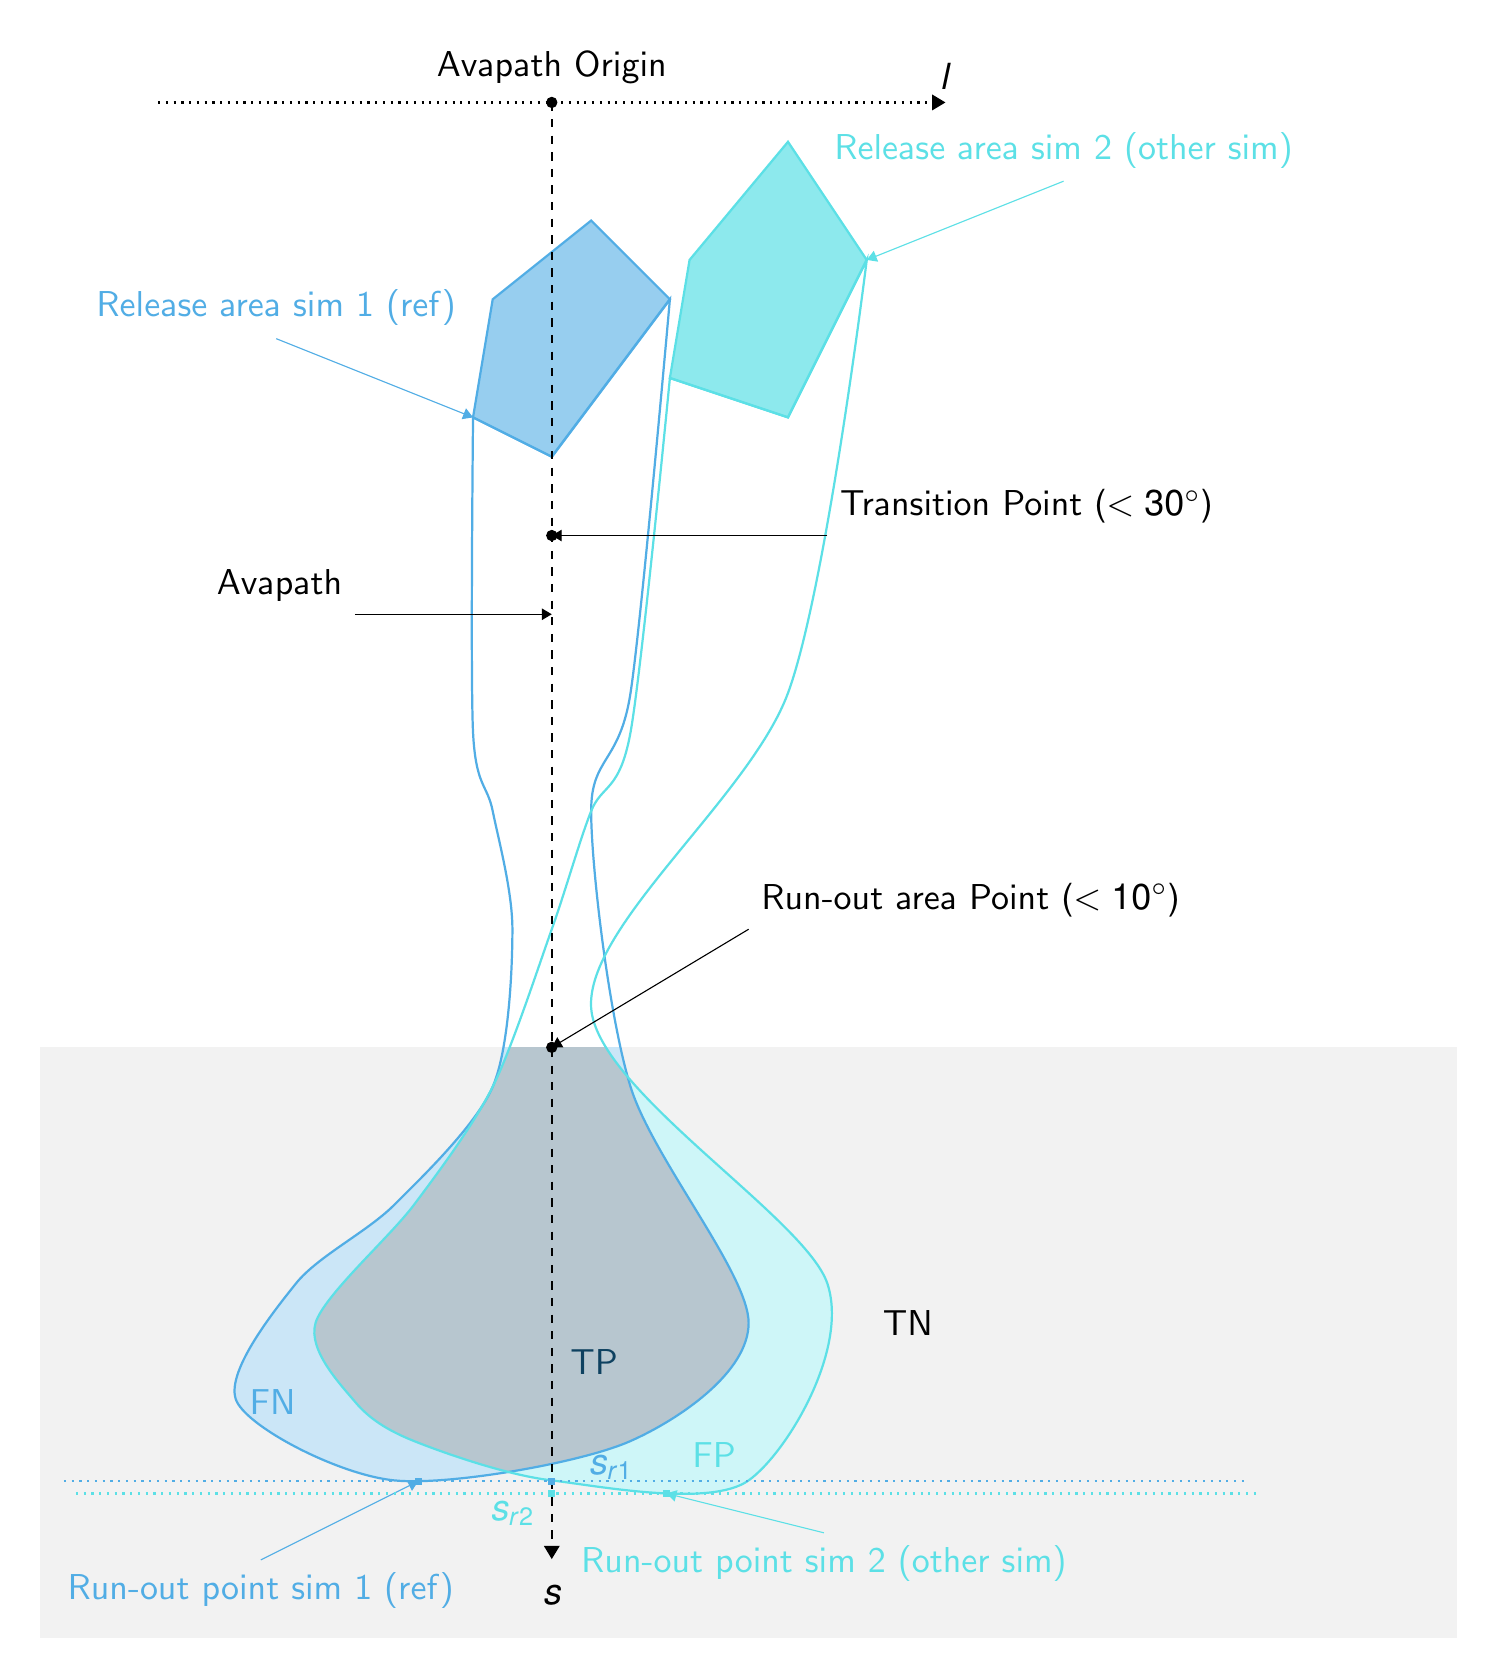
\begin{tikzpicture}[
    scale=0.5,
    every node/.style={scale=1.3},
    >=Triangle,
    show background rectangle,
    background rectangle/.style={fill=white},
    point/.style = {draw, circle,  fill = black, inner sep = 1pt},
    dot/.style   = {draw, circle,  fill = black, inner sep = .2pt},
  ]
% defining coordinates
% reference
\coordinate (RR1) at (-2,25);
\coordinate (RR2) at (-1.5,28);
\coordinate (RR3) at (1,30);
\coordinate (RR4) at (3,28);
\coordinate (RR5) at (0,24);

\coordinate (R1) at (-2,17);
\coordinate (R2) at (-1.5,15);
\coordinate (R3) at (-1,12);
\coordinate (R4) at (-1.5,8);
\coordinate (R5) at (-4,5);
\coordinate (R6) at (-6.5,3);
\coordinate (R7) at (-8,0);
\coordinate (R8) at (-4,-2);
\coordinate (R9) at (2,-1);
\coordinate (R10) at (5,2);
\coordinate (R11) at (2,8);
\coordinate (R12) at (1,15);
\coordinate (R13) at (2,18);


% simulation
\coordinate (RS1) at (3,26);
\coordinate (RS2) at (3.5,29);
\coordinate (RS3) at (6,32);
\coordinate (RS4) at (8,29);
\coordinate (RS5) at (6,25);

\coordinate (S1) at (2,17);
\coordinate (S2) at (1,15);
\coordinate (S3) at (0,12);
\coordinate (S4) at (-1.5,8);
\coordinate (S5) at (-3.5,5);
\coordinate (S6) at (-6,2);
\coordinate (S7) at (-5,0);
\coordinate (S8) at (-3.5,-1);
\coordinate (S9) at (0,-2);
\coordinate (S10) at (5,-2);
\coordinate (S11) at (7,3);
\coordinate (S12) at (1,10);
\coordinate (S13) at (6,18);

% avaPath
\coordinate (O1) at (0,33);
\coordinate (O2) at (0,22);
\coordinate (O3) at (0,20);
\coordinate (O4) at (0,15);
\coordinate (O5) at (0,9);
\coordinate (O6) at (0,0);
\coordinate (O7) at (0,-4);
\coordinate (O8) at (5,-4);
\coordinate (O9) at (-4,-4);


\def\RefAvaRel{
     (RR1) -- (RR2) -- (RR3) -- (RR4) -- (RR5) -- cycle
    }
\def\RefAva{
      plot [smooth] coordinates {(RR1) (R1) (R2) (R3) (R4) (R5) (R6) (R7)  (R8) (R9) (R10) (R11)  (R12) (R13) (RR4)} -- (RR5) -- cycle
    }

\def\SimAva{
     plot [smooth] coordinates {(RS1) (S1) (S2) (S3) (S4) (S5) (S6) (S7)  (S8) (S9) (S10) (S11)  (S12) (S13) (RS4)} -- (RS5) -- cycle
    }
\def\SimAvaRel{
     (RS1) -- (RS2) -- (RS3) -- (RS4) -- (RS5) -- cycle
    }
    

\def\AvaPath{
     (O1) -- (O2) -- (O3) -- (O4) -- (O5) -- (O6) -- (O7)
    }


\begin{scope}
      \fill[black!5] (-13,-6) rectangle (23,9);
\end{scope}
%\draw[black] (-13,-6) rectangle (19,35);
\begin{scope}
      \clip (-10,-5) rectangle (18,9);
      \fill[AFMiddle!30] \RefAva;
\end{scope}
\begin{scope}
      \clip (-10,-5) rectangle (18,9);
      \fill[AFLight!30] \SimAva;
\end{scope}
\begin{scope}
      \clip \RefAva;
      \clip (-10,-5) rectangle (18,9);
      \fill[AFDark!30] \SimAva;
\end{scope}


% Release areas
\draw [thick, AFMiddle, fill=AFMiddle!60] \RefAvaRel;
\draw [thick, AFMiddle, name path=ref ava] \RefAva ;

\draw [thick, AFLight, fill=AFLight!70] \SimAvaRel;
\draw [thick, AFLight, name path=sim ava] \SimAva;

% Avalanche path line
\draw [thick, dashed, black, ->, name path=ava path] \AvaPath;
\node [label=-90:$s$] at (O7) {};
\path [name path=ava path1] (O5) -- (O9);
\path [name path=ava path2] (O6) -- (O8);


\draw [thick, dotted, black, ->] (-10,33) -- (10,33) node[above] {$l$};


\node (origin) at (O1) [point, label = {above:$\mbox{Avapath Origin}$}]{};
\draw[->] (O3) +(-5,0) node[above left] {$\mbox{Avapath}$} -- (O3);
\draw[->] (O2) +(7,0) node[above right] {$\mbox{Transition Point }(<30^\circ)$} -- (O2);
\node (transition) at (O2) [point]{};
\draw[->] (O5) +(5,+3) node[above right] {$\mbox{Run-out area Point }(<10^\circ)$} -- (O5);
\node (runout) at (O5) [point]{};


\draw[->, AFMiddle] (RR1) +(-5,2) node[above] {$\mbox{Release area sim 1 (ref)}$} -- (RR1);
\draw[->, AFLight] (RS4) +(5,2) node[above] {$\mbox{Release area sim 2 (other sim)}$} -- (RS4);

\draw[AFMiddle] (R7) node[right] {$\mbox{FN}$};
\draw[AFLight] (S10) node[above left] {$\mbox{FP}$};
\draw[AFDark] (2,1) node[left] {$\mbox{TP}$};
\draw[black] (10,2) node[left] {$\mbox{TN}$};


\path [name intersections={of=ref ava and ava path1,by=RR}];
\node [fill=AFMiddle,inner sep=1pt] at (RR) {};
\draw[->, AFMiddle] (RR) +(-4,-2) node[below] {$\mbox{Run-out point sim 1 (ref)}$} -- (RR);
\draw[thick, dotted, AFMiddle, name path=runout line1] (RR) +(-9,0) -- ++(21,0);
\path [name intersections={of=runout line1 and ava path,by=RRS}];
\node [fill=AFMiddle,inner sep=1pt] at (RRS) {};
\draw[AFMiddle] (RRS) +(1.5,0.35) node {$s_{r1}$};

\path [name intersections={of=sim ava and ava path2,by=RS}];
\node [fill=AFLight,inner sep=1pt] at (RS) {};
\draw[->, AFLight] (RS) +(4,-1) node[below] {$\mbox{Run-out point sim 2 (other sim)}$} -- (RS);
\draw[thick, dotted, AFLight, name path=runout line2] (RS) +(-15,0) -- ++(15,0);
\path [name intersections={of=runout line2 and ava path,by=RSS}];
\node [fill=AFLight,inner sep=1pt] at (RSS) {};
\draw[AFLight] (RSS) +(-1,-0.5) node {$s_{r2}$};

\end{tikzpicture}

\end{document}